\chapter{Onderzoeksresultaten}

\label{Chapter3}

Dit hoofdstuk heeft als doel antwoord te geven op de onderzoeksvraag: \enquote{\hoofdvraagname}.

\section{Huidige situatie}
Deze paragraaf gaat over de deelvraag \enquote{\deelhuidig}

\subsection{Huidige Architectuur}
De huidige website is een combinatie van een PHP \& Symfony back-end API en Content Management Systeem, samen met een React + next.js front-end. De infrastructuur is momenteel gebouwd op Docker(-compose) + Ansible. Bitbucket pipeline wordt gebruikt voor het Continuous Integration / Deployment. 

In figuur \ref{fig:infra} is een component diagram te vinden van de huidige website structuur. De front-en backend structuur bevat 5 docker containers:
\begin{itemize}
	\item \textbf{PHP-FPM} (back-end)
	\item \textbf{Nginx} (front-en backend)
	\item \textbf{Redis} (back-end)
	\item \textbf{NodeJS} (front-end)
	\item \textbf{PostgreSQL} (back-end)
\end{itemize}

\begin{figure}
	\centering
	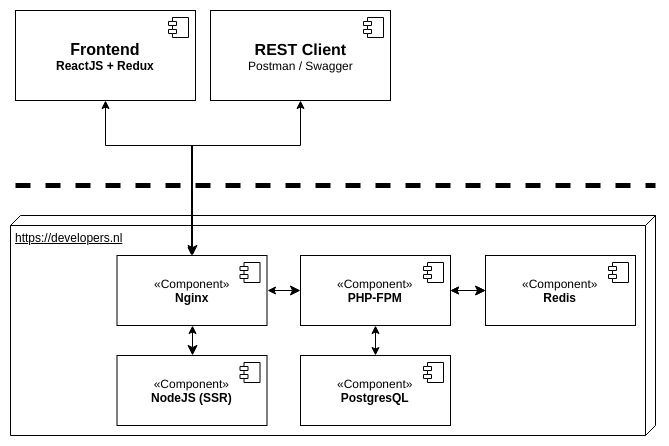
\includegraphics[width=13cm]{Figures/Infrastructure}
	\decoRule
	\caption[Infrastructuur]{Infrastructuur website front-en backend \textbf{HOE CITEREN?}}
	\label{fig:infra}
\end{figure}

PHP-FPM is een FastCGI Process Manager, deze Container serveert de Symfony “FosREST” API en het Content Management Systeem. De NodeJS container serveert een statische Next.js React applicatie en maakt gebruik van Server Side Rendering. Er zit een Nginx reverse proxy in die kiest om een request naar het back-end of de front-end te laten gaan. Redis is een Key-Value Database dat gebruikt wordt voor het cachen, en een PostgreSQL container als database. De Bitbucket Pipeline gebruikt Ansible om op de servers de geüpdatete containers te pullen en te starten.

Voor zowel de front- als backend is één monitoring tool genaamd \enquote{Sentry} geimplementeerd. Sentry creëert een duidelijk overzicht voor alle errors die opkomen in productie.

Ook heeft Developers.nl een \enquote{Employee Management Systeem} (EMS) gebouwd. Deze heeft een soortgelijke structuur aan de website. Het EMS bevat zeer veel gevoelige informatie en het is dus van hoog belang dat deze goed beveiligd is.

\subsection{Metingen}

Nu luidt de vraag, hoe schaalbaar is deze infrastructuur eigenlijk? Om dit te beantwoorden worden de verschillende definities van schaalbaarheid individueel behandeld. 

\subsubsection{Structural scalability}
Definitie: Het vermogen van een systeem om uit te breiden in een gekozen dimensie zonder ingrijpende wijzigingen in de architectuur.


\subsubsection{Load scalability}
Definitie: Het vermogen van een systeem om elegant te presteren naarmate het aangeboden verkeer toeneemt.
\begin{itemize}
	\item https://loader.io/
	\item https://gatling.io/
	\item https://k6.io/
	\item https://loadimpact.com/
	\item http://tsung.erlang-projects.org/
\end{itemize}

Gekozen voor K6 omdat zo goed als elke ontwikkelaar genoeg Javascript kennis heeft om deze tool te gebruiken. Eventueel InfluxDB + Grafana gebruiken voor mooie grafieken.



\subsubsection{Functional scalability}
Definitie: In welke mate bestaande code moet worden aangepast zodra een nieuwe functionaliteit wordt toegevoegd aan het systeem.


\subsection{conclusie}

\section{Technieken}
Deze paragraaf gaat over de deelvraag \enquote{\deeltechnieken}

\section{Verbeteringen}
Deze paragraaf gaat over de deelvraag \enquote{\deelverbetering}


\section{Implementatie}
Deze paragraaf gaat over de deelvraag \enquote{\deelimplementatie}


\section{Requirements}
Deze paragraaf gaat over de deelvraag \enquote{\deelrequirements}